\section{Classifiers}

\subsection{Implementation}

\subsubsection{Mean Euclidean Distance}

\subsubsection{General Euclidean Distance}
The GED classifier is implemented in a similar manner as the MED classifier. However, in the case of GED a whitening transform is applied to the samples to transform them onto a space where features are both uncorrelated, and have unit-variances. This is accomplished using the weighting matrix W. The distance between two points in the transformed space is calculated as,


\begin{eqnarray}
\label{eqn:GED-whitening}
\left [ W=\Lambda^{-1/2}\Phi^{T}  \right ]
\end{eqnarray}



In the above equation, $\Lambda$ contains the eigen values of the covariance matrix $\Sigma$ as elements, and $\Phi$ contains the eigenvectors of $\Sigma$. The simplified distance function is included in \ref{eqn:GED}.

\begin{eqnarray}
\label{eqn:GED}
{d}_{G}(x,z) = {\left [ (x-z)^{T}\Phi\Lambda^{-1/2}\Phi^{T}(x-z) \right ]}^{1/2}
\end{eqnarray}


The decision boundary is therefore calculated in the two- and three- class cases as,

\begin{eqnarray}
\label{eqn:boundary-GED}
& d_{E} (x,z_{1}) = d_{E} (x,z_{2}) \\
& \left [ (x-{z}_{1})^{T}\Phi\Lambda^{-1/2}\Phi^{T}(x-z_{1}) \right ]^{1/2} \\
= & \left [ (x-z_{2})^{T}\Phi\Lambda^{-1/2}\Phi^{T}(x-z_{2}) \right ]^{1/2}  \nonumber \\
&\left [ (x-{z}_{1})^{T}\Phi\Lambda^{-1/2}\Phi^{T}(x-z_{1}) \right ]^{1/2} \\
= &\left [ (x-z_{2})^{T}\Phi\Lambda^{-1/2}\Phi^{T}(x-z_{2}) \right ]^{1/2}  \nonumber \\
= &\left [ (x-z_{3})^{T}\Phi\Lambda^{-1/2}\Phi^{T}(x-z_{3}) \right ]^{1/2}  \nonumber
\end{eqnarray}



In the case of the MatLab implementation, all points on the grid are classified based on identifying the minimum distance between the point and the mean of each class in the transformed space. This allows for a simple contour to be plotted showing the decision boundary between each class. This is shown below for both the two- and three- class case,

\begin{eqnarray}
\label{eqn:pointClass-GED}
min(d_{E} (x,z_{1}), d_{E} (x,z_{2})) \\
min(d_{E} (x,z_{1}), d_{E} (x,z_{2}), d_{E} (x,z_{3}))
\end{eqnarray}


This implementation of the GED classifier and method for creating the decision boundary is shown in Appendix A.

\subsubsection{Maximum A Posteriori}

\subsubsection{Nearest Neighbor}

The nearest neighbor classifier uses MatLab implementation of $knnclassify$. A nearest neighbor classifier will test a point and compare it's distance to all other known classified points. The test point will belong to the class which contains a point with the least ecludian distance to the test point.

The classification boundary is constructed by evaluating many test points on a grid, using the generated data as training data. Due to the nature of nearest neigbor, all training data will be classified correctly; each classified point is it's own nearest neighor.

\begin{figure}[ht]
\centering
	\subfigure[Clusters A, B with NN classification]{
	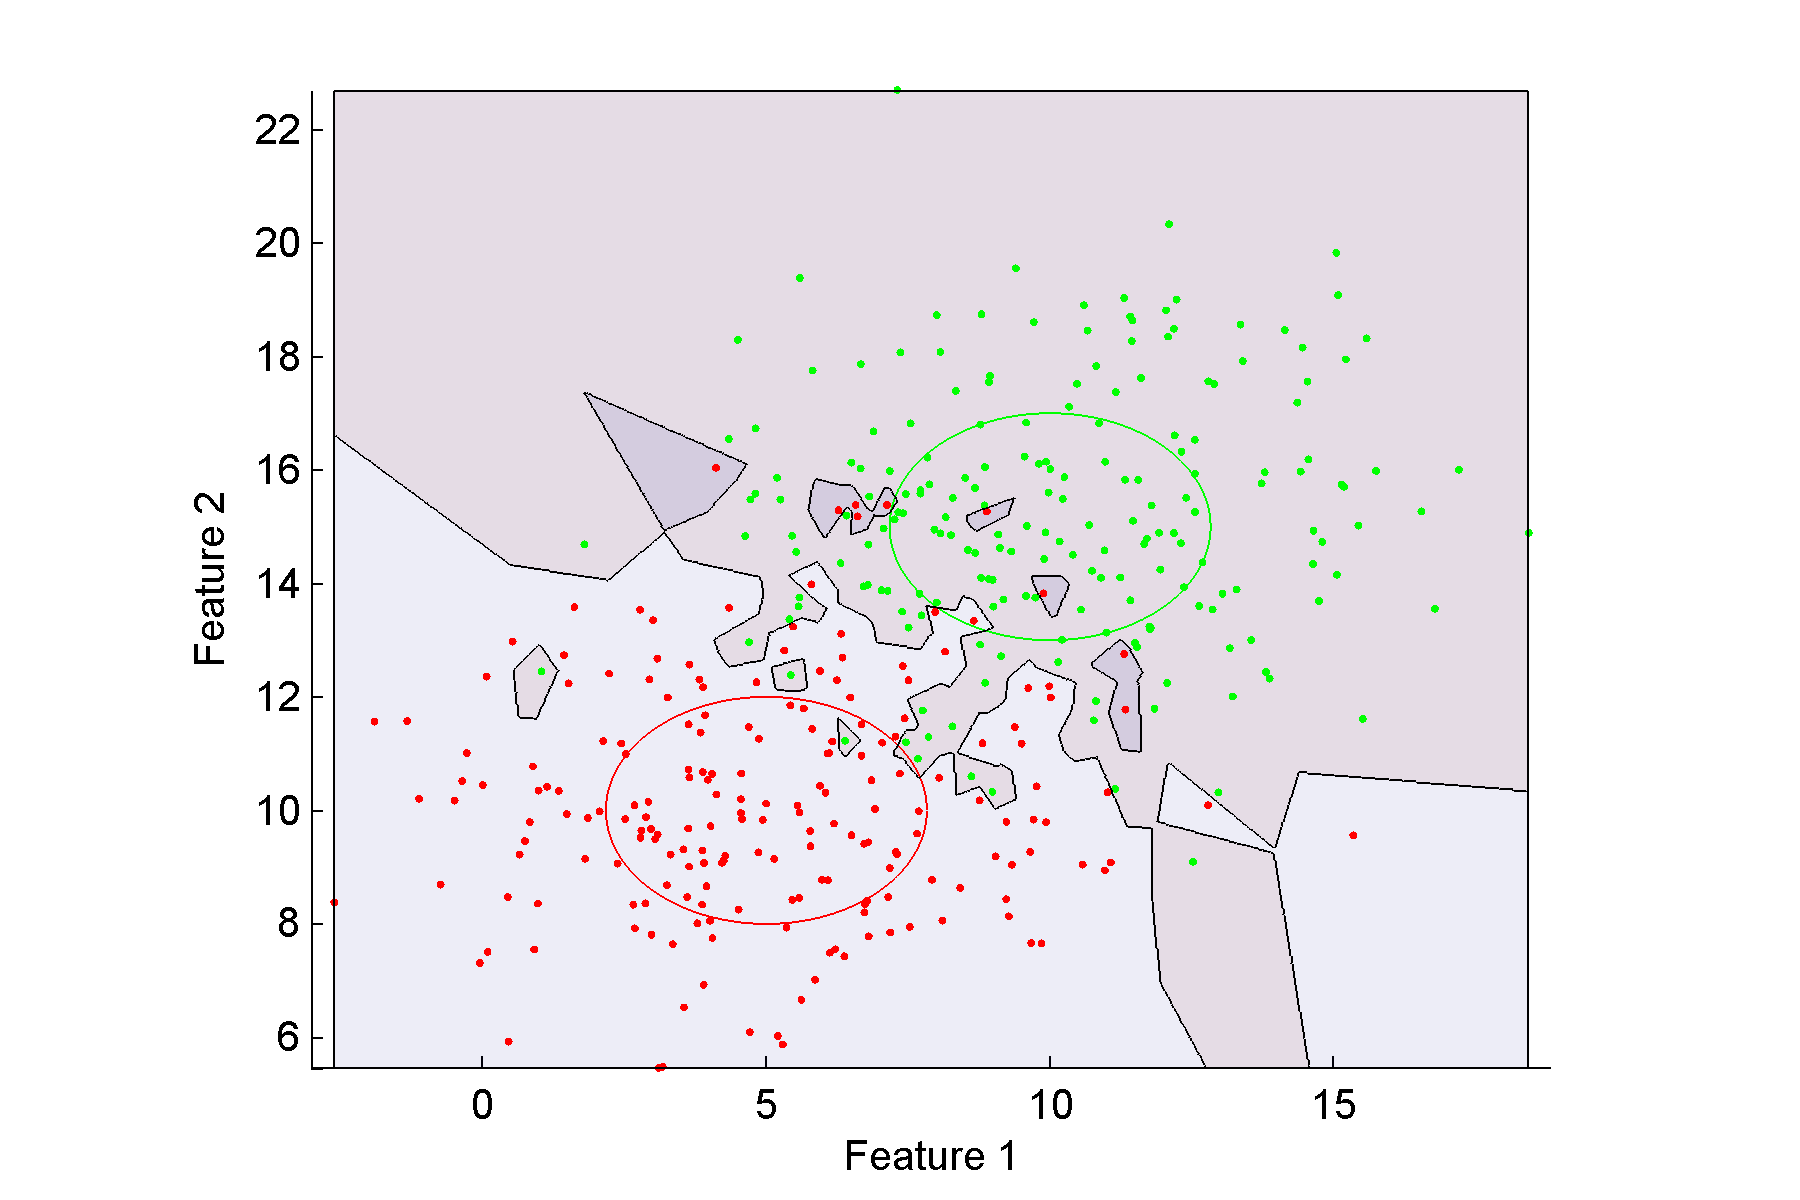
\includegraphics[width=0.45\linewidth]{fig3a-AB_NN}
	}
	\subfigure[Clusters C, D, E with NN classification]{
	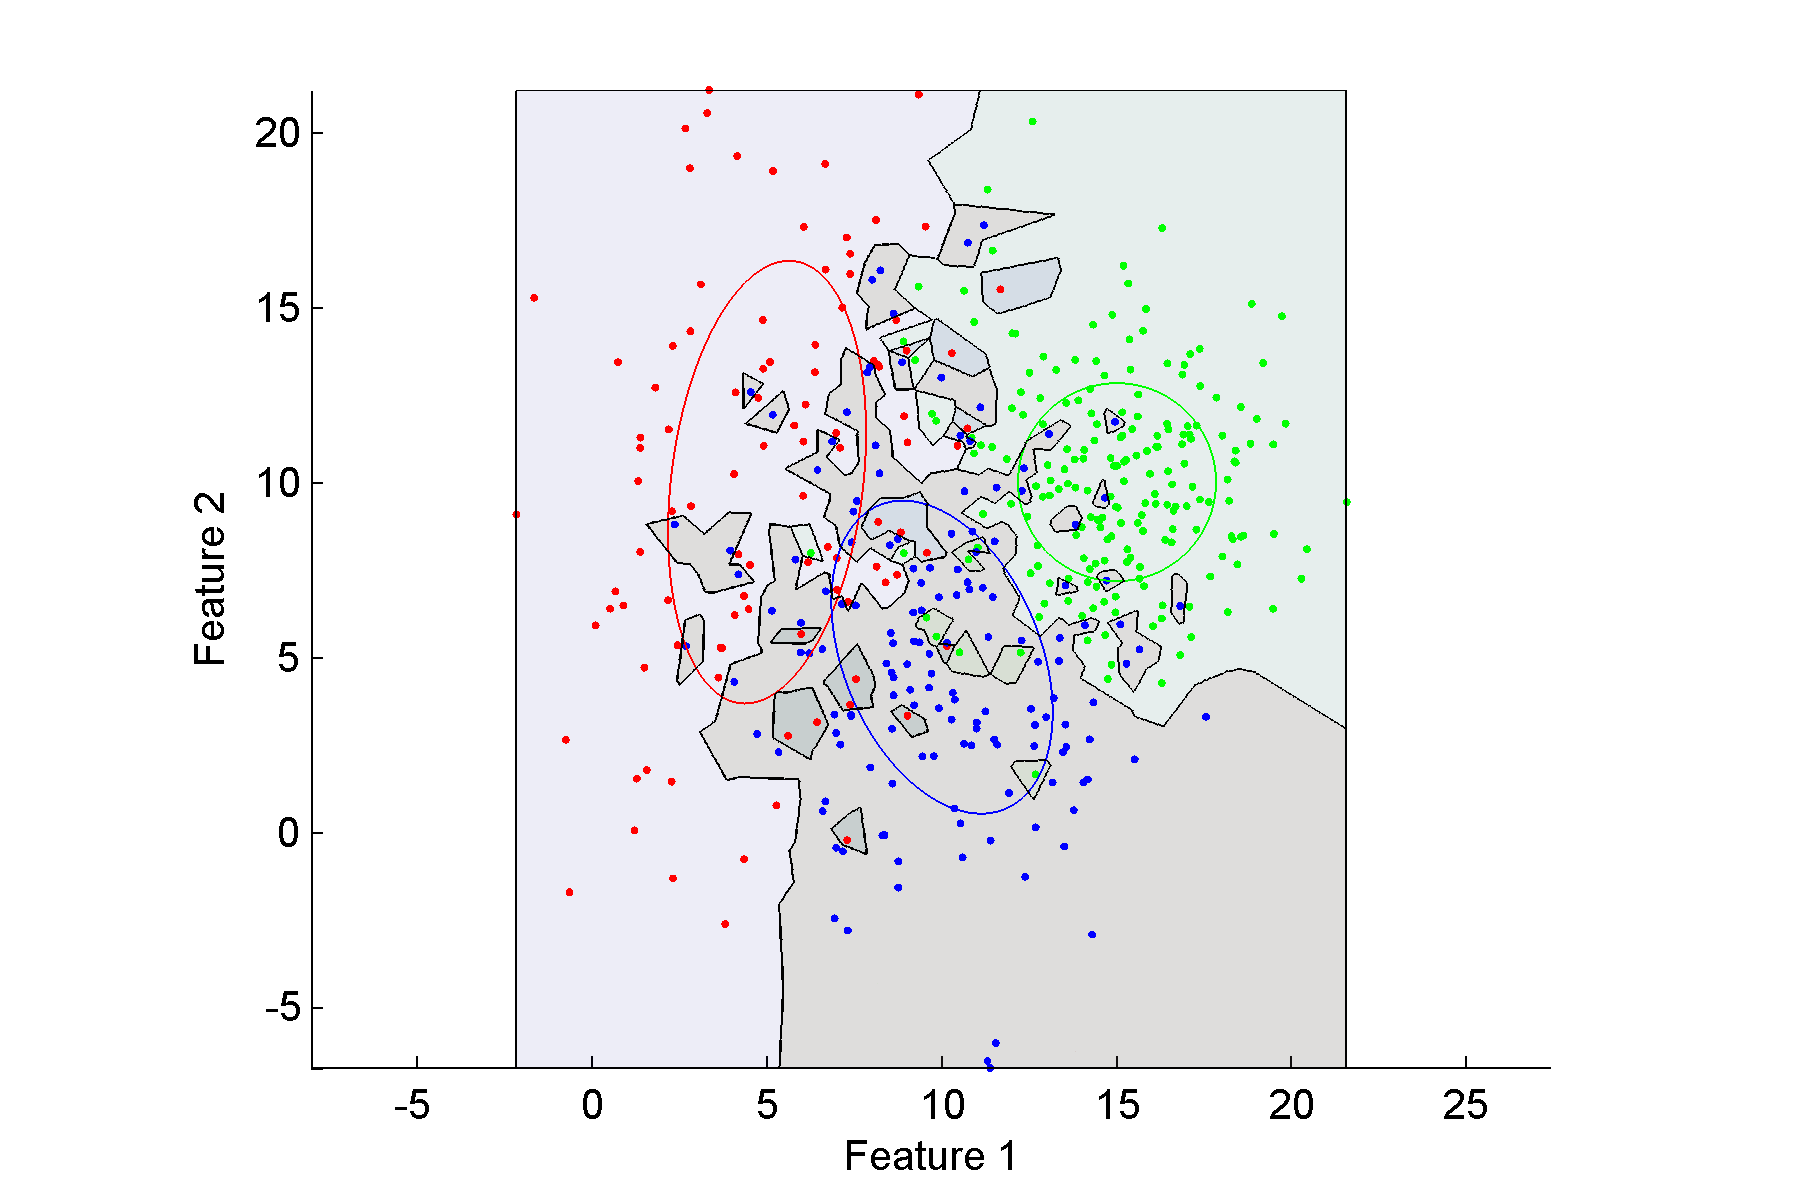
\includegraphics[width=0.45\linewidth]{fig3b-CDE_NN}
	}
	\label{fig:nn_boundary}
	\caption{Nearest Neighbor boundaries}
\end{figure}


\subsubsection{Five Nearest Neighbor}

The nearest neighbor classifier uses MatLab implementation of $knnclassify$. A nearest neighbor classifier will test a point and compare it's distance to all other known classified points. The test point will belong to the class which contains a point with the least ecludian distance to the test point.

The classification boundary is constructed by evaluating many test points on a grid, using the generated data as training data. Due to the nature of nearest neigbor, all training data will be classified correctly; each classified point is it's own nearest neighor.